\documentclass[a4paper,10pt]{report}

\usepackage[utf8x]{inputenc}
\usepackage[francais]{babel}
\usepackage[T1]{fontenc}
\usepackage{graphicx}

\usepackage[colorlinks=true, urlcolor=blue, linkcolor=black]{hyperref}

% Title Page
\title{Web Game Engine - Cahier des charges}
\author{Ilyas Boutebal \and Maxime Colin \and Adrian Gaudebert \and Youness Hamri \and Van-Duc Nguyen}

\begin{document}

  \maketitle
  \tableofcontents

  \chapter{Contexte}

    \section{Le Jeu vidéo}

      Le marché du jeu vidéo s’est beaucoup développé depuis l’arrivée de l’ancêtre Pong ou du célèbre Tetris. On joue aujourd’hui à des jeux de plus en plus beaux, demandant de plus en plus de ressources à nos machines. Mais on voit aussi d’autres utilisations du jeu vidéo arriver : le Serious Gaming, par exemple, est une branche en pleine expansion en ce moment. Le Social Gaming également, représenté activement par les nombreux jeux basés sur Facebook et ses possibilités en terme de diffusion.

      Parmi les différentes ``catégories'' de jeux vidéos, il en est une qui s'est particulièrement développée ces dernières années : les jeux en ligne. Dans cette grande catégorie, on trouve beaucoup de types de jeux différents : les MMO dans le genre de World of Warcraft, les jeux multijoueur comme Counter Strike ou Team Fortress, les modes multi de jeux principalement solo, et les jeux par navigateur.

    \section{Les jeux par navigateur}

      Le jeu par navigateur, ou Browser Game en anglais, se joue par définition dans un navigateur Internet. On retrouve donc dans cette catégorie les jeux “Facebook” cités plus haut, la majorité des jeux en Flash, mais également un très grand nombre de jeux que nous appellerons les Jeux Web, puisqu’ils se basent sur les technologies du Web ouvert. Quelques exemples de jeux web relativement connus : Ogame, Travian, ou le français Hordes.

      Ces trois exemples ne sont cependant pas représentatifs de la diversité que l’on trouve dans les jeux web. Les jeux d’élevage virtuel, par exemple, sont extrêmement nombreux sur le Web. À quoi est due cette profusion de jeux web ? Majoritairement à la simplicité d’accès du développement web. Faire un jeu web, en soit, c’est développer un site web. Or, avec des technologies très répandues comme PHP, HTML et CSS, avec toutes les ressources que l’on trouve autour de ces dernières (il suffit de regarder les tutoriels du Site du Zéro pour s’en rendre compte), il est très simple pour une personne un peu motivée de créer son propre jeu web.

      Malheureusement, s’il est simple de créer un jeu web “basique”, les développeurs sont rapidement limités par les technologies qu’ils utilisent. Il est quasiment impossible de faire du temps réel avec PHP, le couple HTML / CSS n’est pas adapté à l’affichage d’effets spéciaux ou d’animations complexes, et si l’arrivée récente de frameworks JavaScript comme jQuery a permis de repousser un peu ces limites techniques, cela ne résout pas le problème.

    \section{Les technologies du web}

      Il existe une solution simple aux limitations techniques actuelles des technologies web : se tourner vers le futur et utiliser de nouvelles technologies, pas encore éprouvées, mais qui permettent d’aller beaucoup plus loin dans la création de nos jeux web.

      HTML 5, la nouvelle mouture du langage de description des pages web, apporte au développeur un très grand nombre de fonctionnalités clés : le temps réel dans le navigateur avec les WebSockets, les manipulations graphiques avancées avec le SVG et les Canvas, la vidéo et le son avec Video et Audio, et bien d’autres.

      La version 3 du langage CSS offre elle aussi d’alléchantes nouveautés : les animations, les transitions, les polices particulières, ainsi que tous les effets graphiques amplement simplifiés.

      Toutes les avancées actuelles du web ouvrent indéniablement les portes à des jeux de plus en plus impressionnants, de plus en plus profonds, le tout se passant dans un navigateur ! Il faudra cependant du temps pour que les développeurs maîtrisent tout ceci, pour que des outils facilitant l’utilisation de ces technologies apparaissent, et donc pour que l’accès à toutes ces possibilités pour nos jeux devienne simple.

    \section{Besoin}
    
      Ce besoin est bien réel : le projet Fightly\footnote{\url{http://fightly-dev.lqbs.fr/forum/}}, par exemple, vise à créer un jeu de stratégie au tour par tour bénéficiant directement de ces avancées. La création d'un outil fournissant un ensemble de fonctionnalités de base, facilitant l'accès aux technologies Web récentes et simplifiant donc largement le développement d'un tel projet ne pourra que mener à une amélioration globale de ce jeu.

      Fightly est un jeu de stratégie au tour par tour dans lequel des joueurs s'affrontent en manipulant des unités. Les parties se déroulent sur des cartes à cases hexagonales, les unités s'y déplaçant en fonction du terrain et des stratégies des joueurs. Les joueurs choisissent au début de la partie leurs unités, composées de fantassins, archers ou chevaliers, chacunes ayant des caractéristiques et des capacités différentes. Le jeu se déroule en temps et en tours limités, le gagnant étant le dernier joueur en vie, ou à défaut celui ayant le plus de points. 
      
      Il existe également le jeu Alonya\footnote{\url{http://alonya.eu/}}, qui reprend largement le concept des jeux Civilization en l'adaptant au Web (et en ajoutant quelques modifications bien sur). Ce jeu est actuellement en développement, et n'utilisera donc a priori pas notre moteur, mais l'existance d'un tel outil aurait certainement aidé la création d'Alonya. 



  \chapter{Le projet}

    \section{Objectifs}

      Voici donc où se place ce projet : notre objectif est de fournir un outil complet, permettant de créer de façon simple et rapide un jeu profitant des dernières avancées en matière de technologie web. Il constituera un ensemble d'outils qui fournissent un cadre de développement et des fonctionnalités permettant d'implémenter tout ou partie d'un jeu.

      Le moteur sera prioritairement conçu pour des jeux de stratégie au tour par tour. On cherchera à le rendre aussi générique que possible, afin de permettre une grande diversité dans les types de jeux développables avec notre outil. On veillera aussi à faciliter l'extensibilité du projet, toujours dans le but d'offrir la possibilité d'en étendre facilement les fonctionnalités.

      Un des objectifs secondaires du projet est d'utiliser des technologies récentes et innovantes. Si la compatibilité avec les différents navigateurs du marché doit être un facteur important, elle ne doit pas être une limitation dans le choix des outils à utiliser. 

      Pour finir, ce projet sera libre, c'est-à-dire qu'il sera distribué sous licence libre, et qu'à terme on voudra mettre en place une communauté autour du développement de ce produit. 


    \section{Les jeux de stratégie au tour par tour}

      L'objectif de ce projet est de permettre la création de jeux de stratégie au tour par tour : on va donc étudier ce type de jeux pour en dégager les grands concepts, les particularités, les éléments nécessaires. Nos choix se sont portés sur les jeux suivants : 

      \begin{itemize}
        \item Dofus : MMORPG dont le module de combat est en tour par tour
        \item Civilization : Jeu de gestion d'un empire
        \item Heroes of Might and Magic : Jeu de campagnes militaires, univers médiéval / fantastique
        \item Battle for Wesnoth : Jeu d'aventure, univers médiéval / fantastique
        \item Fightly
      \end{itemize}

      Les diagrammes représentant les concepts de ces jeux, ains que des informations complémentaires, sont disponibles dans l'Annexe A. De ces jeux, nous avons donc trouvé un ensemble de concepts qui reviennent, et composent donc a priori la base de tout jeu de stratégie au tour par tour. Certains de ces éléments n'ont pas forcément le même nom selon le jeu, et des différences au niveau de l'implémentation peuvent apparaitre, mais on peut les généraliser en un concept plus global. 

      Voici donc le diagramme modélisant les concepts qui nous paraissent essentiels à la réalisation d'un jeu de stratégie au tour par tour : 
      
      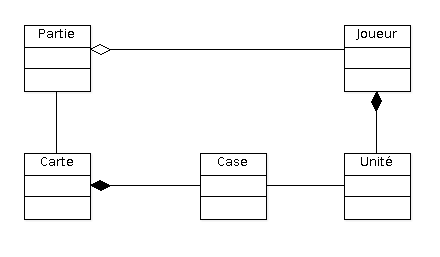
\includegraphics[width=320px]{diagrammes/concept-fightly.png}



    \section{Spécifications}

      L'objectif de ce projet est de créer un moteur de jeu web : on utilisera donc naturellement une architecture Client / Serveur. 

      La partie Serveur devra être mise en place sur un serveur dédié. Elle prendra en charge les règles du jeu, les parties et leur état (appelé le ``Monde''), les joueurs. Elle gérera également la communication avec les clients. Cette partie devra donc, la majorité du temps, recevoir des demandes d'action de la part d'un joueur, valider cette action par rapport aux règles et à l'état du Monde de la partie concernée, puis valider cette action et répercuter les changements induits chez tous les joueurs. On devra également gérer la mise en place d'une partie (par exemple, dans le jeu Fightly, il faut attendre d'autres joueurs, puis chaque joueur créé une armée, puis chaque joueur place son armée sur la carte, et enfin le jeu commence ``réellement'') et la fin d'une partie (calcul du gagnant, actions particulières en fonction du jeu). 
      
      Cependant, on ne s'occupera pas dans cette partie Serveur de tout ce qui correspondrait au rôle d'un serveur web classique. Par exemple, on n'assurera pas la distribution des fichiers statiques (c'est-à-dire HTML, CSS, JavaScript et images), ni la création et configuration des parties. On considère que, lorsqu'un joueur rejoint une partie, il a déjà tous les éléments nécessaires à sa gestion. Nous estimons que ces fonctionnalités ne rentrent pas dans le cadre d'un moteur de jeu, et qu'elles ne trouvent donc pas leur place dans ce projet. De plus, ce sont des fonctionnalités classiques, que de nombreux outils gèrent. On pourra donc facilement coupler notre moteur de jeu à un autre outil assurant toutes les fonctions. On pourra également envisager d'ajouter ces responsabilités au moteur par la suite. 

      La partie Client correspond à ce qui est exécuté dans le navigateur du joueur. Cette application gérera donc l'affichage du jeu chez le joueur, ainsi que les interactions avec ce dernier. L'application cliente devra pouvoir communiquer avec le serveur, mais également avec d'autres clients (typiquement, les autres joueurs présents dans une partie en cours). En règle générale, cette partie enverra des demandes d'action au serveur, et appliquera en local les changements qui lui sont ordonnés par ce même serveur. 


  \chapter{Conception}

    \section{Architecture générale}

      Le diagramme suivant présente les principaux modules qui composeront la partie serveur de notre application. 
      
      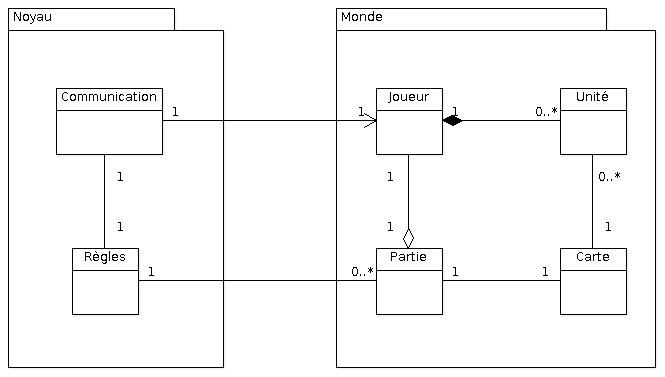
\includegraphics[width=320px]{diagrammes/moteur_serveur_classes.png}
      
      Les modules de la partie cliente sont représentés dans le diagramme suivant. 
      
      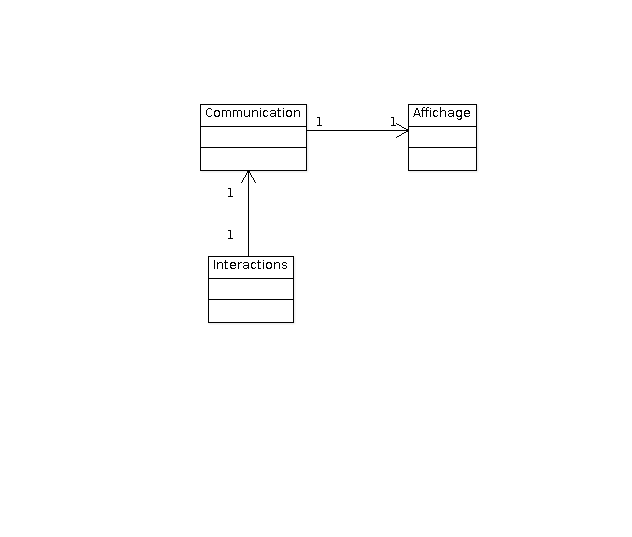
\includegraphics[width=320px]{diagrammes/moteur_client_classes.png}


    \section{Serveur}

      Le serveur sera la partie du moteur qui fera tourner les parties et permettra la communication et les interactions entre les joueurs. Il aura pour rôle de contrôler les parties, lier les clients et gérer leur actions. Il aura également le rôle d'arbitre dans une partie. 

      Le serveur sera séparé en deux grandes parties : une partie Noyau et une partie Monde.

      \subsection{Package Noyau}

        La partie Noyau du serveur gère les fonctionnalités de base du moteur. Elle contient un ensemble de modules qui sont a priori indépendants du type de jeu implémenté. L'objectif principal de ce package est de faire le lien entre les actions du joueur et la représentation centralisée du Monde\footnote{Rappel : on appelle ``le Monde'' l'ensemble des données représentant l'état d'une partie.} d'une partie. On trouve donc deux parties principales, une gérant les liens avec les clients, l'autre s'occupant des règles et du lien avec la gestion du Monde. 

        Le module communication du serveur prend en charge tous les échanges réseau avec les clients. Elle s'occupe d'accepter les nouvelles connexions, fait l'association entre client (au sens réseau) et joueur (au sens du jeu), et permet donc de recevoir des messages d'un joueur ainsi que de lui en envoyer. Ce module aura aussi à charge la gestion des déconnexions éventuelles de joueurs. 

        Le module règles sera chargé de stocker et de traiter les règles du jeu. Il contiendra des fonctionnalités permettant de créer une base de règles. Ces règles pourront être ajoutées ou supprimées individuellement ou chargées à partir d'un fichier de règles. La partie règle devra également valider (ou invalider) les actions demandées par les joueurs, en fonction des règles connues et de l'état du Monde.

      \subsection{Package Monde}

        La partie Monde est composée d'un ensemble de modules qui gèrent les fonctionnalités principales d'un jeu de stratégie au tour par tour. On y retrouvera donc les notions que l'on a dégagées des différents jeux étudiés (cf. partie 2.2 Les jeux de stratégie au tour par tour), et que l'on considère comme étant primordiales pour tout jeu STpT\footnote{STpT : Stratégie au Tour par Tour}. 
        
        Ce package devra être le plus générique et le plus extensible. On devra pouvoir modifier facilement le comportement des modules sans que cela n'affecte les autres. De plus, on devra pouvoir ajouter de nouvelles fonctionnalités, et les intégrer au moteur.

        Dans ce package Monde, on trouvera quatre modules principaux. Tout d'abord, un module représentera les parties, en permettant de les charger depuis un support de persistence. Il gérera également les tours, l'ordre des joueurs, et toute la configuration particulière qu'une partie peut avoir. 

        Le deuxième module concernera les joueurs : on les caractérisera pour les différencier, et chaque joueur possèdera un ensemble d'unités qui pourra manipuler. On stockera également les points gagnés par le joueur durant la partie. 

        Un troisième module sera dédié à la gestion de la carte. Celle-ci sera composée d'un ensemble de cases, chacune de ces cases étant caractérisée par plusieurs paramètres, comme l'accessibilité ou l'influence sur les unités qui s'y trouvent. 

        Enfin, on aura un module pour représenter les unités. Une unité possèdera un ensemble de paramètres (par exemple, une valeur offensive, une valeur défensive, une vie... ), appartiendra à un unique joueur et sera à tout moment sur une seule case. Une unité détruite sera supprimée de la partie, et donc retirée de l'état du Monde. 


    \section{Client}

      La partie cliente de notre moteur de jeu sera exécutée dans le navigateur du joueur. Cette partie devra donc gérer l'affichage du jeu, les actions de l'utilisateur et les communications avec le serveur ou avec les autres joueurs. 

      \subsection{Affichage}

        L'application cliente devra posséder une représentation du Monde contenant, au minimum, les données nécessaires au bon affichage du jeu. Ainsi, les notions de Carte, Joueur ou Unité devront se trouver sur le client, sous une forme simplifiée, limitée à la gestion des états. 
        
        Dans le navigateur du client, on voudra pouvoir afficher des informations sur la partie (nombre de tour restants, temps restant dans le tour, joueur actif... ) et sur les joueurs présents dans la partie. La carte sera affichée sous la forme d'un ensemble de cases contigues, les unités des joueurs seront représentées sur ces cases. 
        
        En plus des fonctionnalités nécessaires à la bonne gestion de la représentation du Monde, on voudra fournir des outils permettant de simplifier la création d'effets graphiques, comme par exemple des animations lors du déplacement d'une unité, ou lors d'un combat entre deux unités ennemies. Le but est de permettre au développeur de créer rapidement des effets avancés pour son jeu, afin de le rendre plus attractif. 

      \subsection{Interactions}

        L'application cliente est en rapport direct avec le joueur, elle devra donc s'occuper de traiter les actions que le joueur demande d'effectuer. Chaque action de l'utilisateur deviendra une demande d'action, qui sera envoyée par la partie Communication au(x) destinataire(s) de la demande (serveur ou autres joueurs). 
        
        Par exemple, on devra gérer le clic sur un bouton qui demande à finir le tour si le joueur est actif. Ou on enverra aux autres joueurs un message rédigé sur le chat de la partie. 
        
        Comme pour la partie Affichage, on mettra en place des outils permettant d'interagir de manière poussée avec l'interface du jeu. On pourra par exemple vouloir déplacer une unité par un système de drag & drop. 

      \subsection{Communication}

        Le module de Communication de l'application cliente aura deux rôles principaux. D'accord, se connecter au serveur ou à d'autres joueurs, et leur envoyer des demandes d'actions. Mais aussi, et surtout, recevoir et traiter des demandes d'actions en provenance de ces derniers. Les messages envoyés par le serveur sont des ordres, et devront donc être appliqués directement : la partie Communication devra pouvoir demander des modification sur l'état du Monde du client, ces modifications impliquant bien sur un raffraichissement de l'affichage. 


  \chapter{Livrables intermédiaires}

    On fournira au client trois livrables intermédiaires au cours du projet

    \section{Veille technologique}

      On effectuera, dans un premier temps, une veille technologique afin d'étudier l'existant et de déterminer quels sont les meilleurs choix de technologies à utiliser pour ce projet. 

      Date de rendu : 17 décembre 2010.

    \section{Dossier d'analyse}

      Il sera important d'écrire un dossier de conception détaillé, présentant tous les aspects techniques du projet, les problématiques et les solutions envisagées. Ce dossier servira de base au développement du projet, et devra être validé par le client. 

      Date de rendu : 7 janvier 2011.

    \section{Version de démonstration}

      On voudra, à la moitié de la phase de développement, fournir au client une version de démonstration au client. Cette application consistera en un simple client ``spectateur'', qui ne fera donc rien d'autre qu'afficher le Monde d'une partie. Le client pourra donc valider ou imputer nos choix à ce moment, et nous permettre de corriger certaines erreurs éventuelles avant la fin du projet. 

      Date de rendu : 19 janvier 2011. 



  \chapter{Livrables finaux}

    À la fin du projet, on fournira au client les trois éléments suivants : 

    \begin{list}{-}{}
      \item{Le code source complet de l'application développée ;}
      \item{Une documentation technique, à destination des développeurs qui utiliseront le moteur, mais également à l'intention des développeurs qui contribueront par la suite au projet, celui-ci étant libre ;}
      \item{Une démonstration technique du moteur.}
    \end{list}

    Date de rendu : 4 février 2011.



  \chapter{Organisation}

    \section{Décomposition générale}

      Décomposition du projet en modules

      \begin{list}{-}{}
        \item{Serveur}
        \begin{list}{-}{}
          \item{Noyau}
          \begin{list}{-}{}
            \item{Communication}
            \item{Règles}
          \end{list}
          \item{Monde}
          \begin{list}{-}{}
            \item{Partie}
            \item{Joueur}
            \item{Carte}
            \item{Unité}
          \end{list}
        \end{list}

        \item{Client}
        \begin{list}{-}{}
          \item{Affichage}
          \item{Communication}
          \item{Interactions}
        \end{list}
      \end{list}


    \section{Responsabilités}

      La conduite du projet sera assurée par Adrian. Il aura par ailleurs à développer le module Affichage de la partie Client. 

      Maxime sera responsable de la partie Serveur, il devra donc en contrôler le bon avancement, la cohérence et la qualité au fur et à mesure du développement. Il sera également en charge du développement du module de Règles. 

      Le package Noyau du serveur sera sous la responsabilité de Duc, qui devra donc en assurer le suivi, et qui développera le module Communication de ce même noyau, ainsi que celui de la partie Client. 

      Le package Monde sera pris en charge par Youness. Il devra également développer les modules Partie, Joueur et Carte du Serveur. 

      Enfin, la partie Client sera sous la responsabilité de Ilyas, qui en développera également le module Interactions. Il développera aussi le module Unité du package Monde du serveur. 


    \section{Planning}

      Planning


\appendix

\chapter{Jeux de stratégie au tour par tour}

	\section{Civilization}

		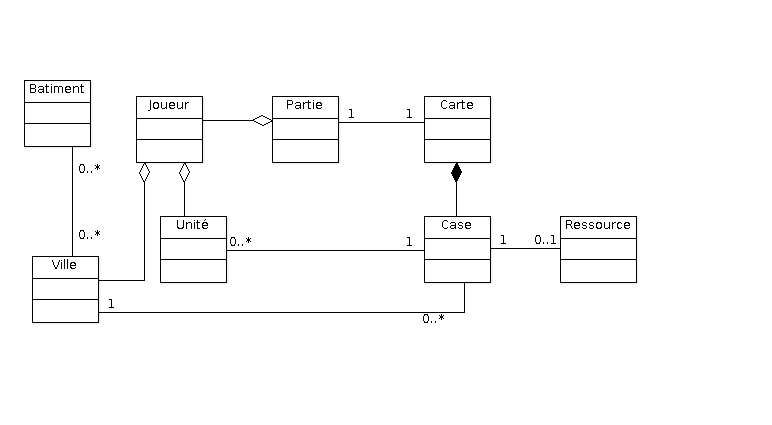
\includegraphics[width=320px]{diagrammes/concept_civilization.png}


	\section{Dofus}
	
		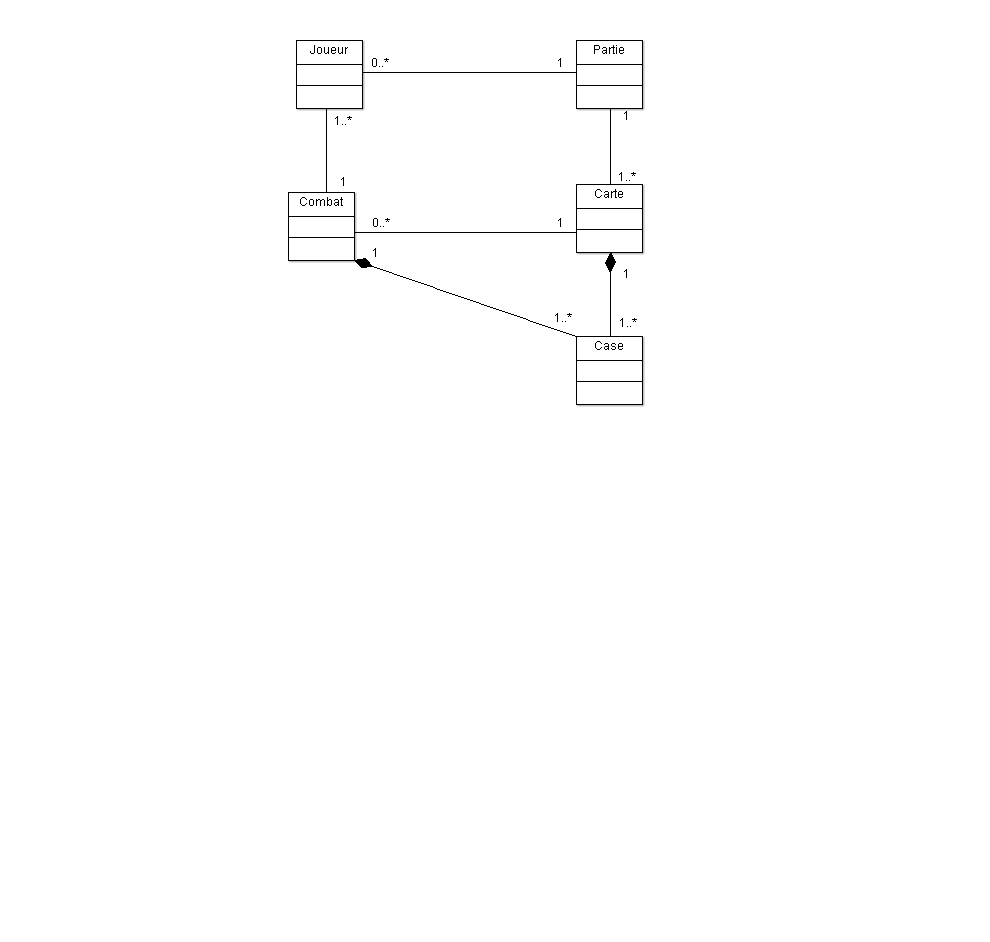
\includegraphics[width=320px]{diagrammes/classdiagram_dofus.png}
     
		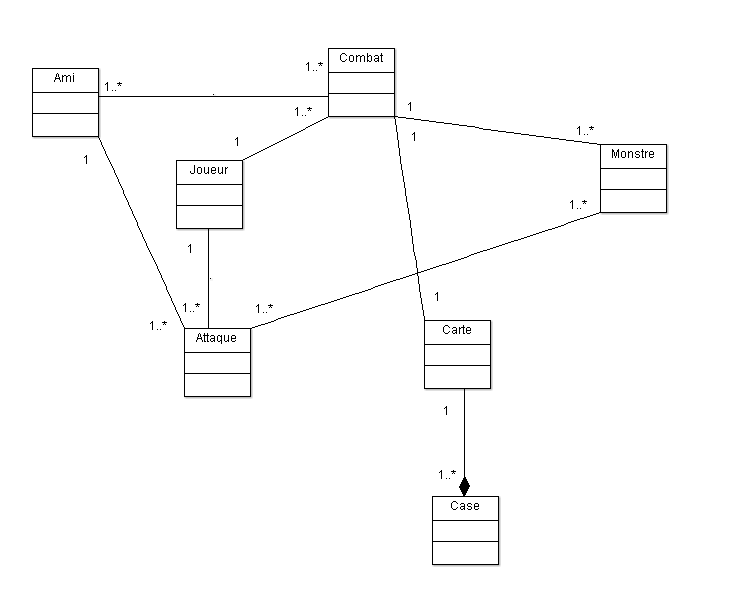
\includegraphics[width=320px]{diagrammes/concept_dofus.png}


	\section{Heroes of Might and Magic}
	
    Diagramme de classes présentant les principaux concepts du jeu : 
    
		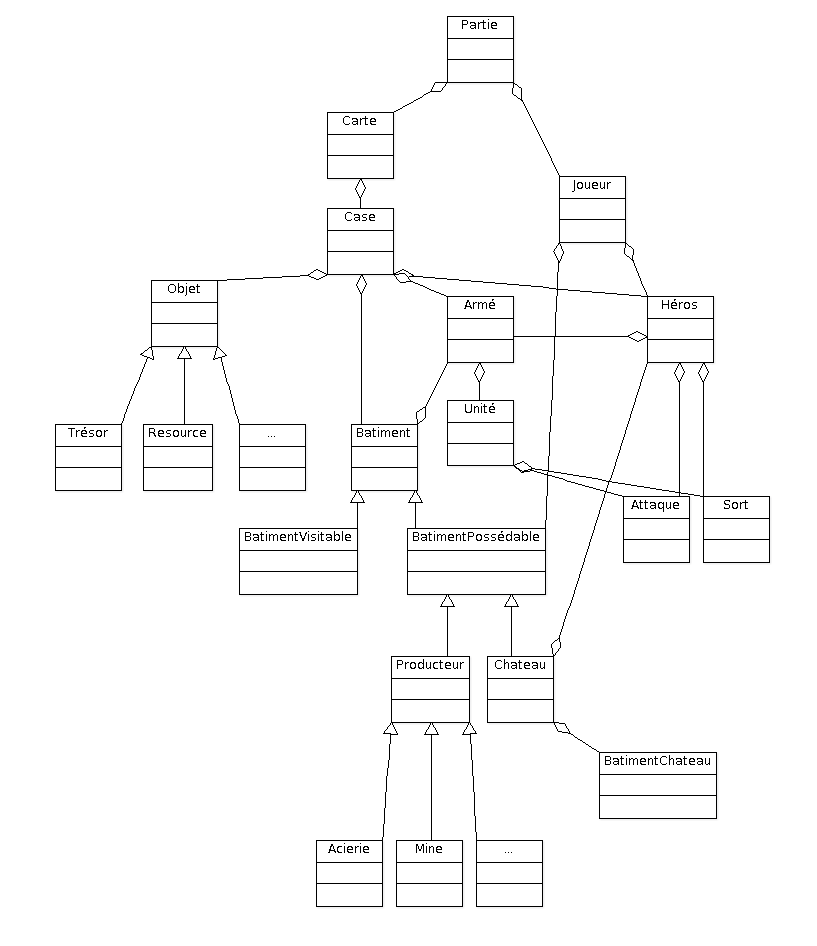
\includegraphics[width=320px]{diagrammes/heroes_of_might_and_magic.png}

    Diagramme d'activités présentant le déroulement global du jeu : 
    
    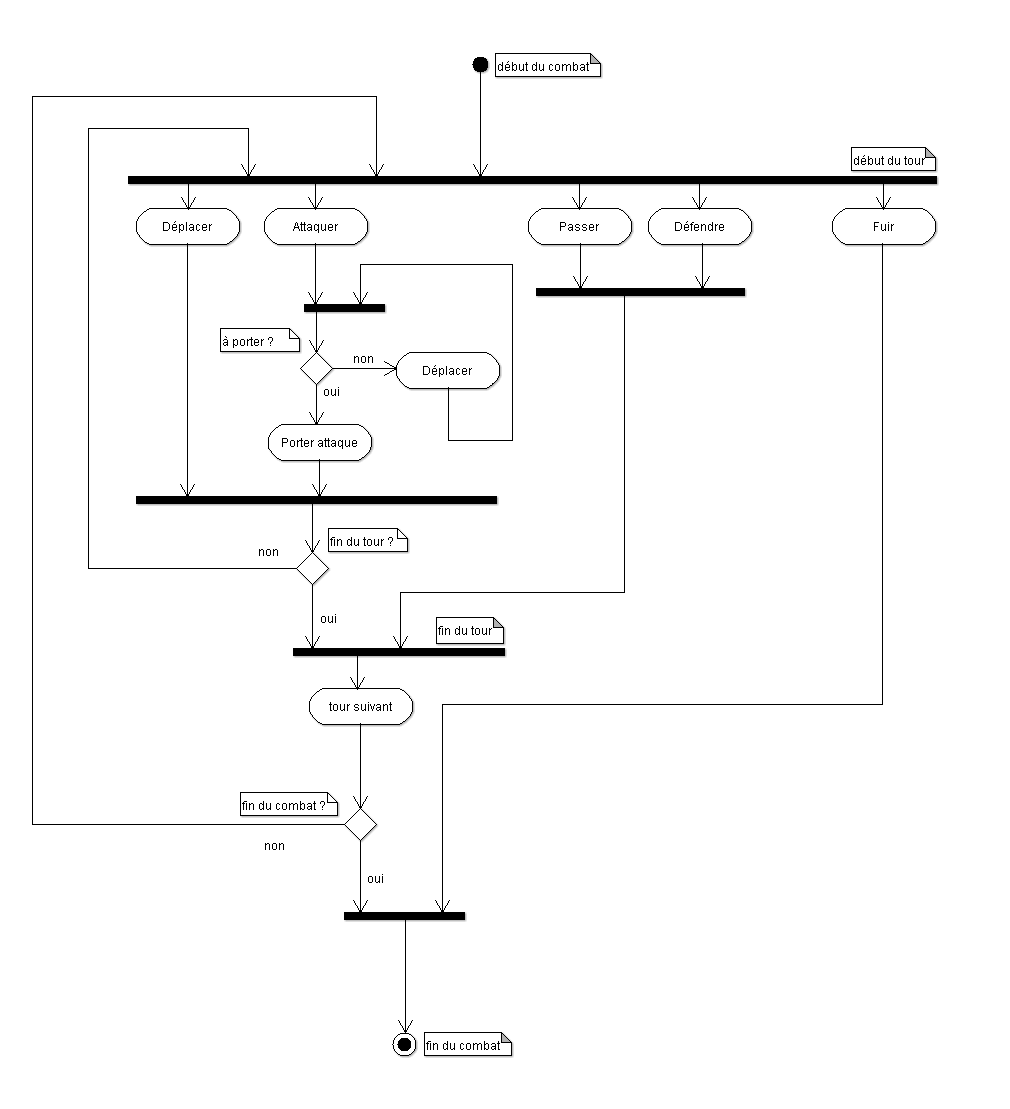
\includegraphics[width=320px]{diagrammes/sequence-homm.png}


	\section{Battle for Wesnoth}
	
		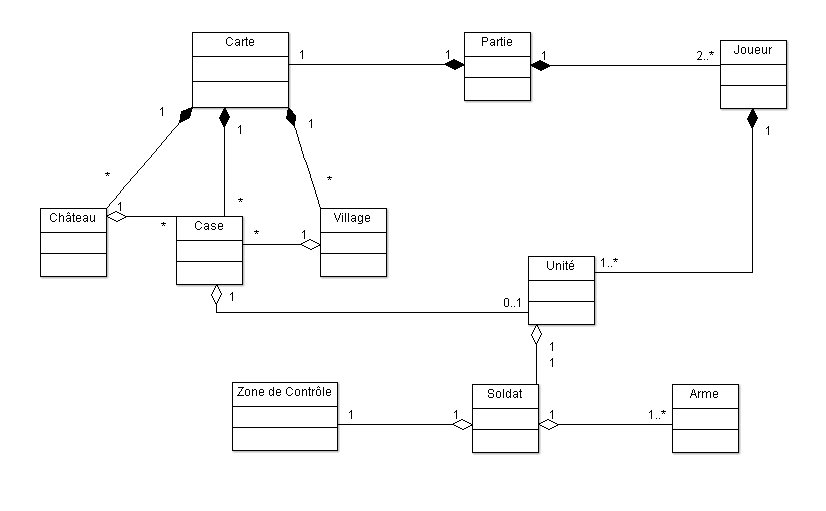
\includegraphics[width=320px]{diagrammes/Concept-Battle-of-Wesnoth.png}


	\section{Fightly}
	
		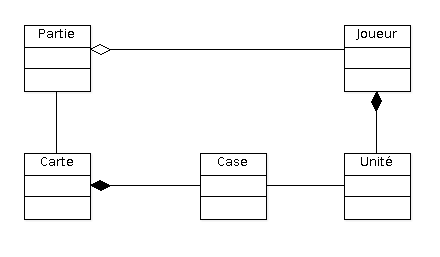
\includegraphics[width=320px]{diagrammes/concept-fightly.png}


\end{document}
